\begin{minipage}[l]{0.5\textwidth}
  \begin{exerciseS}[Gradiente di pressione in tubi cilindrici]
  Si deve progettare un condotto che trasporti un fluido con densità
  $\rho_1$ e viscosità $\mu_1$, di diametro $d_1$ e lunghezza $L_1$.
  Si suppone che la rugosità della superficie interna del condotto possa
  essere descritta interamente dall'altezza media $\epsilon_1$
  delle asperità. Il condotto deve garantire una portata massica $Q_1$.
  Viene realizzato un modello in scala $\lambda = d_2 / d_1$ del condotto
  di lunghezza $L_2$, nel quale viene fatto scorrere lo stesso fluido 
  alle stesse condizioni termodinamiche. Si chiede di determinare:
  \begin{itemize}
   \item la finitura superficiale della superficie interna del modello,
         in termini di dimensione caratteristica della rugosità $\epsilon_2$;
   \item la velocità media di prova $U_2$;
   \item la differenza di pressione da imporre alle estremità del condotto
         al vero, conoscendo che la differenza di pressione $\Delta P_2$
         misurata in laboratorio.
  \end{itemize}
  Si supponga il fluido incomprimibile.
  \end{exerciseS}

\end{minipage}
\hspace{3mm}
\begin{minipage}[r]{0.5\textwidth}
 \centering
  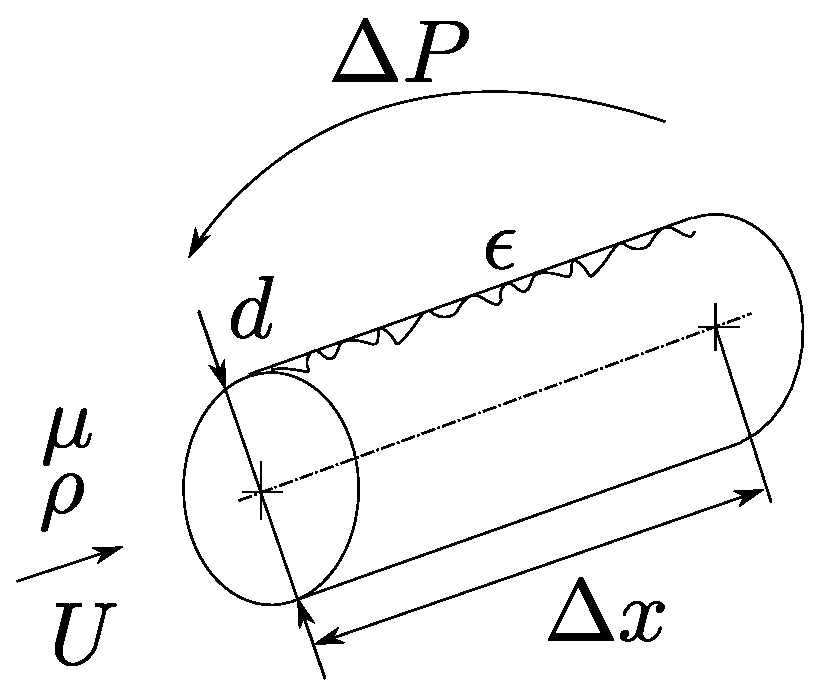
\includegraphics[width=1.0\textwidth]{./fig/pipe}
\end{minipage}

\sol

\partone
 Teorema di Buckingham. Similitudine fluidodinamica.

\parttwo
Il problema è caratterizzato dal fluido utilizzato, dalla geometria del
 condotto e dal gradiente di pressione necessario a garantire la portata
 desiderata. Si può scrivere in maniera implicita
 \begin{equation}
  f\left( \dfrac{\Delta P}{\Delta x}, U, \rho, \mu, d, \epsilon \right) = 0
 \end{equation}
 avendo scelto come grandezza fisica caratteristica del problema il
  gradiente di pressione $\dfrac{\Delta P}{\Delta x}$ e non il salto di
  pressione e la lunghezza del tubo prese indipendentemente.
 Il teorema di Buckingham garantisce che il problema può essere
  caratterizzato da 3 numeri adimensionali (6 grandezze fisiche - 3 grandezze
  fondamentali (M,L,T)). Se si scelgono $\rho$, $U$, $d$ come grandezze di
  riferimento, si possono costruire i tre numeri adimensionali come
  \begin{equation}
   \pi_1 = \dfrac{\Delta P}{\Delta x} \dfrac{d}{\rho U^2} = f_D \qquad
   \pi_2 = \dfrac{\mu}{\rho U d} = 1/Re \qquad
   \pi_3 = \dfrac{\epsilon}{d} = \epsilon'
  \label{eqn:pi}
  \end{equation}
 Il problema può essere quindi scritto in forma implicita come:
 \begin{equation}
  g(f_D,Re,\epsilon') = 0.
 \end{equation}
 Esplicitando $f_D$:
 \begin{equation}
  f_D = h(Re,\epsilon') \qquad
  \dfrac{\Delta P}{\Delta x} = \dfrac{\rho U^2}{d} f_D(Re,\epsilon').
 \end{equation}
 Affinchè sia verificata la similitudine fluidodinamica, ci deve essere
 l'uguaglianza dei numeri di Reynolds $Re$ e delle rugosità
 adimensionalizzate $\epsilon'$.
 
 \begin{itemize}
  \item Dall'uguaglianza delle rugosità adimensionalizzate
    \begin{equation}
      \epsilon'_1 = \epsilon'_2=:\epsilon' \quad \Rightarrow \quad \epsilon_2 = \epsilon_1 \dfrac{d_2}{d_1} = \lambda \epsilon_1.
    \end{equation}
    Per il modello è quindi necessaria una lavorazione che garantisca una
     finitura superficiale migliore rispetto al condotto al vero
     ($\lambda \le 1$).
  \item La velocità media al vero $U_1$ viene ricavata grazie alla richiesta
   dellaportata desiderata.
     \begin{equation}
       U_1 = \dfrac{Q}{\rho \frac{\pi}{4} d_1^2}
     \end{equation}
     Per ottenere la similitudine fluidodinamica si impone l'uguaglianza
     dei numeri di Reynolds
     \begin{equation}
      Re_1 = Re_2=:Re \quad \Rightarrow \quad U_2 = U_1
       \dfrac{\rho_1 d_1 \nu_2}{\rho_2 d_2 \nu_1} = U_1 \dfrac{d_1}{d_2}
     \end{equation}
     poichè la densità e la viscosità del fluido ``di prova'' sono le stesse
     di quelle del fluido ``al vero''.
  \item Il rapporto tra la differenza di pressione $\Delta P_2$ misurata sul
   condotto modello e la lunghezza del condotto modello $L_2$ permette di
   stimare il gradiente di pressione $\dfrac{\Delta P}{\Delta x}\Big|_2 =
   \dfrac{\Delta P_2}{L_2}$.
   Sfruttando ancora una volta la similitudine fluidodinamica
   \begin{equation}
   \begin{cases}
    \dfrac{\Delta P_2}{L_2} = \dfrac{\rho_2 U_2^2}{d_2} f_D(Re,\epsilon') \\
    \dfrac{\Delta P_1}{L_1} = \dfrac{\rho_1 U_1^2}{d_1} f_D(Re,\epsilon') \\
   \end{cases}
    \Rightarrow \Delta P_1 = \Delta P_2 \dfrac{\rho_1 U_1^2}{\rho_2 U_2^2}
     \dfrac{d_2}{d_1} \dfrac{L_1}{L_2}
   \end{equation}
   Dall'uguaglianza delle densità $\rho_1/\rho_2 = 1$; dall'uguaglianza dei
   numeri di Reynolds (e delle densità e viscosità) $	U_1^2/U_2^2 =
   d_2^2/d_1^2$. La formula può quindi essere semplificata
   \begin{equation}
     \Delta P_1 = \Delta P_2 \dfrac{d^3_2}{d^3_1} \dfrac{L_1}{L_2} =
                  \Delta P_2 \lambda^3 \dfrac{L_1}{L_2}
   \end{equation}
 \end{itemize}

\paragraph{Diagramma di Moody.} Il diagramma di Moody riporta il 
 coefficiente $f_D$ in funzione del numero di $Re$ e della rugosità
 del tubo.
 Si possono individuare due regimi estremi del problema. Per ``basse
  velocità'' (o meglio, bassi numeri di Reynolds), si può intuire che gli
  effetti  della viscosità prevalgano sugli effetti inerziali; inoltre, gli
  effetti della rugosità sono minimi.
  Si può quindi pensare che il problema sia indipendente dalla densità
  del fluido e dalla rugosità del tubo e descrivibile in forma implicita 
  come
  \begin{equation}
    f_L (\Delta P / \Delta x, \mu, U, d) = 0
  \end{equation}
  Si può descrivere il problema solo con un numero adimensionale. Scegliendo
  $\mu$, $U$, $d$ come grandezze di riferimento, si può scrivere
  \begin{equation}
   \pi_{1,L} = \dfrac{\Delta P}{\Delta x} \dfrac{d^2}{\mu U}
  \end{equation}
  Il problema può essere scritto in forma implicita $g_L(\pi_{1,L}) = 0$. 
  Poichè la funzione $g_L$ dipende solo dal coefficiente $\pi_{1,L}$, il
  coefficiente $\pi_{1,L}$ deve essere costante. Il gradiente di pressione
  può essere scritto 
  \begin{equation}
    \dfrac{\Delta P}{\Delta x} = \pi_{1,L} \dfrac{\mu U}{d^2} = 
      \dfrac{\rho U^2}{d} f_D
  \end{equation}
  avendo usato la definizione di $f_D$ introdotta nell'equazione
  (\ref{eqn:pi}). \'E quindi possibile stimare l'andamento del coefficiente
  $f_D$, per bassi numeri di Reynolds, invertendo l'equazione precedente. Si
  scopre che il coefficiente $f_D$ è inversamente proporzionale al numero 
  di Reynolds.
  \begin{equation}
   f_D = \pi_{1,L} \dfrac{\mu}{\rho U d} = \pi_{1,L} \dfrac{1}{Re}
  \end{equation}.
  Per bassi numeri di Reynolds, il parametro $f_D$ in funzione di $Re$
  mostra un andamento lineare in un diagramma con assi logaritmici, a
  conferma della correttezza della stima appena svolta.
  
  Si può ragionare in maniera analoga per il regime di moto estremo opposto,
  dove gli effetti della viscosità sono trascurabili. Si scopre
  che il coefficiente $f_D$ è funzione solo della rugosità adimensionale
  $\epsilon$, mentre non dipende dal numero di Reynolds.
  Per alti numeri di Reynolds, il parametro $f_D$ è descritto da curve che
  tendono a un valore costante, che dipende dal valore della rugosità
  adimensionale $\epsilon'$.

\begin{minipage}[r]{1.0\textwidth}
 \centering
  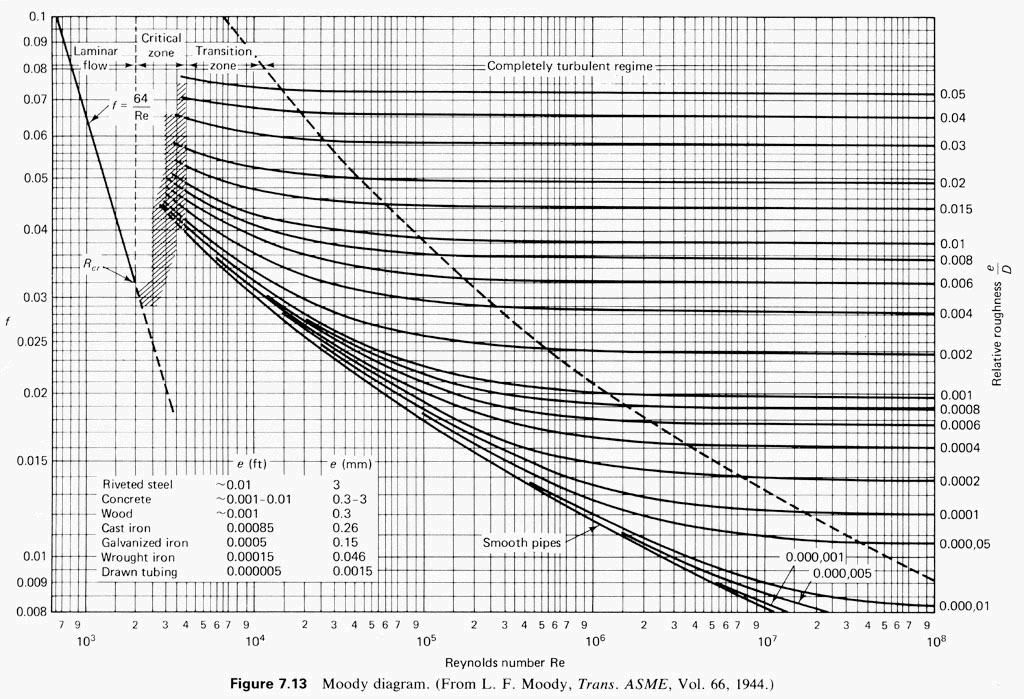
\includegraphics[width=1.0\textwidth]{./fig/MoodyChart.jpg}
\end{minipage}

